\documentclass[11pt, titlepage]{article}
\usepackage{amsmath,amsthm,amssymb}
\usepackage{hyperref, pgf, tikz}
\usepackage{fancyhdr}
\usetikzlibrary{arrows}
\usepackage[margin=1.25in]{geometry}
\usepackage{graphicx}                     
\pagestyle{fancy}
\usepackage{array}
\usepackage{indentfirst}
%\usepackage{wrapfig}

\lhead{Lab \#3}
\rhead{\thepage}
\cfoot{}

\title{The RC Time Constant \\ \ \\ \large Lab \#3}
\author{Name: Avery Karlin \\ Partner: Jeffrey Zou}
\date{}
\begin{document}

\maketitle

\begin{center}
\LARGE The RC Time Constant
\end{center}

\section*{Objective}
The objective of the lab is to measure the time constant of an RC circuit based on the rate of charging and discharging.

\section*{Introduction}
Capacitors are defined by the equation $Q = CV$, such that the voltage of the capacitor is directly proportional to the charge, with the proportionality constant called the capacitance. Similar, resistor voltage is defined by Ohm's Law, such that $V = IR$. Thus, for a circuit purely with a resistor and a capacitor (RC circuit), the differential equation by Kirchoff's Voltage Law states that for charging (connected to the battery), $V_0 = \frac{Q}{C} + R\frac{dQ}{dt}$, and when discharging (disconnected from the battery), $0 = \frac{Q}{C} + r\frac{dQ}{dt}$. Thus, this can be solved to get an equation for charging, $V = V_0(1 - e^{\frac{-t}{RC}}) = V_0(1 - e^{\frac{-t}{\tau}}$ and for discharging, $V = V_0e^{\frac{-t}{RC}} = V_0e^{\frac{-t}{\tau}}$, where $\tau = RC$, called the time constant for an RC circuit.

These equations can be modified such that for charging, $-ln(\frac{V_0 - V}{V_0}) = -\frac{t}{RC}$ and for discharging, $-ln(\frac{V}{V_0}) = -\frac{t}{RC}$. Since the left-hand side here forms a constant term and the right is a constant multiplied by t, it forms a line with the slope equal to $\frac{-1}{RC}$.

\section*{Procedures and Results}

First, the power source is connected to a capacitor and then a variable resistor set to some value, joined back to the power source, with a voltmeter connected to the capacitor to measure the capacitor's charging voltage. After the power source is activated, it is timed with a stopwatch as it charges, recording the voltage as time increases, until the voltage of the capacitor is negligibly less than the battery, and it can't increase further. After, it is disconnected from the power source, such that the resistor is directly connected to the capacitor, such that it acts as the power source, discharging as voltage is lost through the resistor, recording the voltage as time increases again until it has only a negligible amount of voltage remaining. This is then repeated for a capacitor of a different capacitance.

\begin{figure}[h]
\centering
\hspace*{0cm}
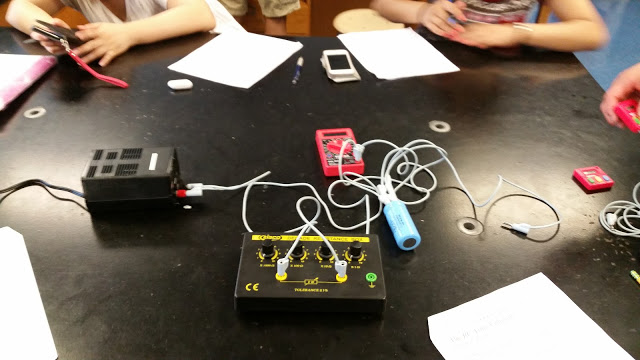
\includegraphics[scale=0.6]{lab31.jpg}
\vspace*{0cm}
\end{figure}

\begin{figure}[h]
\centering
\hspace*{0cm}
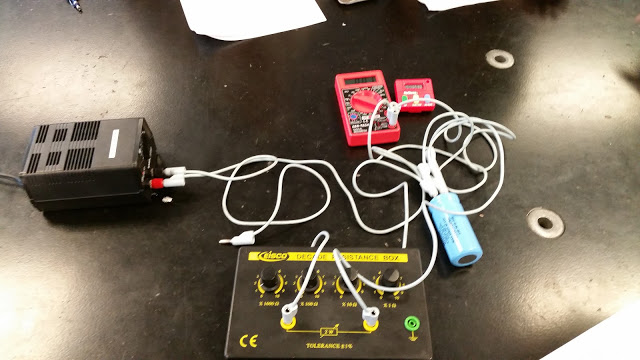
\includegraphics[scale=0.6]{lab32.jpg}
\vspace*{0cm}
\end{figure}

\underline{Capacitor 1:}
\begin{center}
$$C = 5100 \mu F$$
$$R = 1350 \Omega$$
\begin{tabular}
{|m{9em}|m{9em}|m{9em}|}
\hline
Charging Time (s) & Charging Voltage (V) & Discharging Voltage (V) \\
\hline
0 & 0 & 8.87\\
\hline
4 & 3.48 & 5.48\\
\hline
8 & 5.47 & 3.37\\
\hline
12 & 6.8 & 2.12\\
\hline
16 & 7.53 & 1.43\\
\hline
20 & 8.06 & 0.9\\
\hline
24 & 8.31 & 0.6\\
\hline
28 & 8.51 & 0.38\\
\hline
32 & 8.63 & 0.26\\
\hline
36 & 8.72 & 0.17\\
\hline
40 & 8.77 & 0.12\\
\hline
\end{tabular}
\end{center}

\underline{Capacitor 2:}
\begin{center}
$$C = 4200 \mu F$$
$$R = 1350 \Omega$$
\begin{tabular}
{|m{9em}|m{9em}|m{9em}|}
\hline
Charging Time (s) & Charging Voltage (V) & Discharging Voltage (V) \\
\hline
0 & 0 & 8.91\\
\hline
4 & 5.18 & 4.74\\
\hline
8 & 7.16 & 2.30\\
\hline
12 & 7.84 & 1.13\\
\hline
16 & 8.26 & 0.6\\
\hline
20 & 8.60 & 0.33\\
\hline
24 & 8.75 & 0.16\\
\hline
28 & 8.81 & 0.10\\
\hline
32 & 8.87 & 0.06\\
\hline
36 & 8.89 & 0.03\\
\hline
40 & 8.90 & 0.02\\
\hline
\end{tabular}
\end{center}

\section*{Discussion}
Sample calculations for the non-measured data are as shown using the formulas found above:

$$\text{Average Slope (Capacitor 1)} = \frac{\text{Charging Slope} + \text{Discharging Slope}}{2} = \frac{-0.108 - 0.11}{2} = -0.109 1/F*s$$
$$RC \text{(Measured, Capacitor 1)} = \frac{-1}{\text{Average Slope}} = \frac{-1}{-0.109} = 9.174 F*s$$
$$RC \text{(Calculated, Capacitor 1)} = R*C = 5100*10^-6*1350 = 6.885 F*s$$
$$\text{Percent Error (Capacitor 1)} = \frac{\text{$|$Expected - Actual$|$} * 100\%}{\text{Expected}} = \frac{|6.885 - 9.174| * 100\%}{6.885} = 33.2\%$$

\underline{Capacitor 1:}
\begin{center}
$V_0 = 8.87 V$
\begin{tabular}
{|m{6em}|m{6em}|m{6em}|m{6em}|}
\hline
Charging Time (s) & Charging $V_0 - V$ & Charging $ln(V_0 - V)$ & Discharging $ln(V)$ \\
\hline
0 & 8.87 & 2.18 & 2.18\\
\hline
4 & 5.39 & 1.68 & 1.7\\
\hline
8 & 3.4 & 1.22 & 1.21\\
\hline
12 & 2.07 & 0.73 & 0.75\\
\hline
16 & 1.34 & 0.29 & 0.36\\
\hline
20 & 0.81 & -0.21 & -0.11\\
\hline
24 & 0.56 & -0.58 & -0.51\\
\hline
28 & 0.36 & -1.02 & -0.97\\
\hline
32 & 0.24 & -1.43 & -1.35\\
\hline
36 & 0.15 & -1.9 & -1.77\\
\hline
40 & 0.10 & -2.3 & -2.12\\
\hline
\end{tabular}
$$\text{Charging Slope} = -0.11 1/F*s$$
$$\text{Discharging Slope} = -0.108 1/F*s$$
$$\text{Average Slope} = -0.109 1/F*s$$
$$RC \text{(Measured)} = 9.174 F*s$$
$$RC \text{(Calculated)} = 6.885$$
$$\text{Percent Error} = 33.2\%$$
\end{center}

\begin{figure}[h]
\centering
\hspace*{0cm}
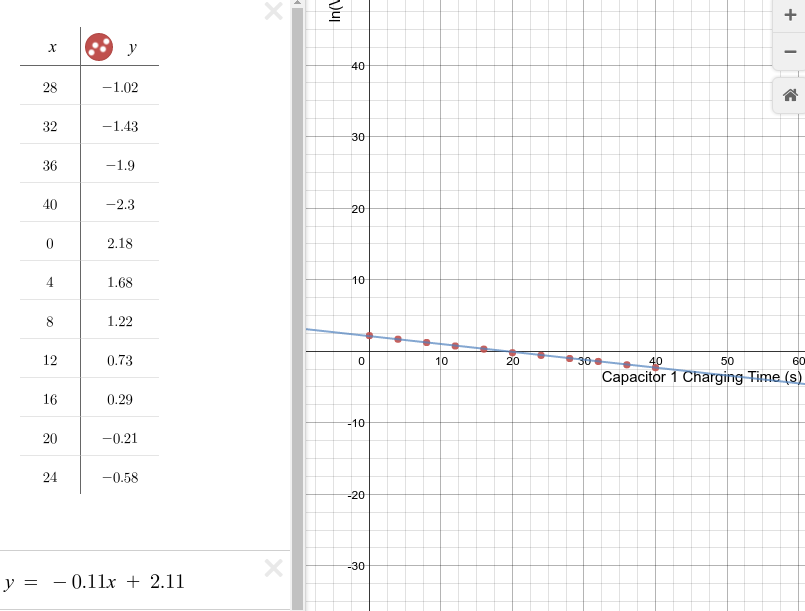
\includegraphics[scale=0.6]{graph31.jpg}
\vspace*{0cm}
\end{figure}

\begin{figure}[h]
\centering
\hspace*{0cm}
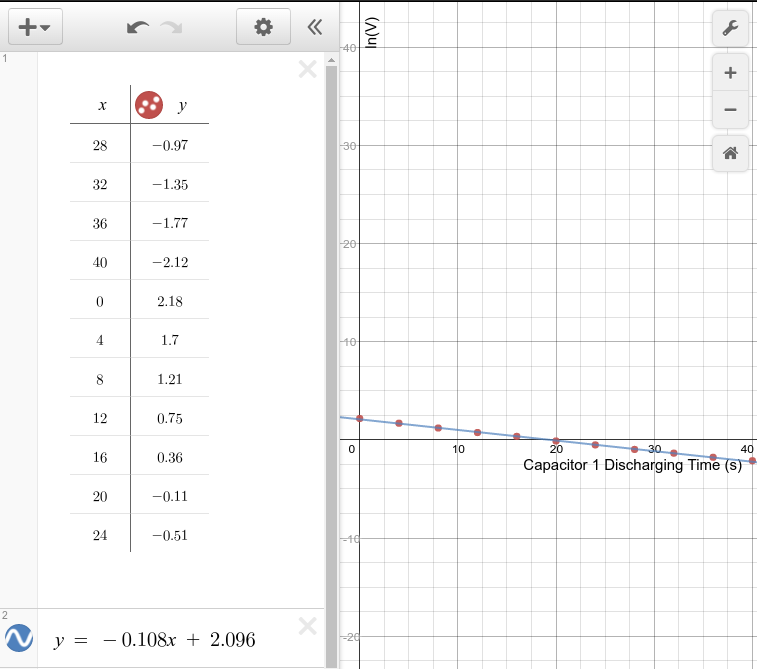
\includegraphics[scale=0.6]{graph32.jpg}
\vspace*{0cm}
\end{figure}

\underline{Capacitor 2:}
\begin{center}
$V_0 = 8.91 V$
\begin{tabular}
{|m{6em}|m{6em}|m{6em}|m{6em}|}
\hline
Charging Time (s) & Charging $V_0 - V$ & Charging $ln(V_0 - V)$ & Discharging $ln(V)$ \\
\hline
0 & 8.91 & 2.19 & 2.19\\
\hline
4 & 3.73 & 1.32 & 1.56\\
\hline
8 & 1.75 & 0.56 & 0.83\\
\hline
12 & 1.07 & 0.07 & 0.12\\
\hline
16 & 0.65 & -0.43 & -0.51\\
\hline
20 & 0.31 & -1.17 & -1.11\\
\hline
24 & 0.16 & -1.83 & -1.83\\
\hline
28 & 0.1 & -2.3 & -2.3\\
\hline
32 & 0.04 & -3.22 & -2.81\\
\hline
36 & 0.02 & -3.91 & -3.5\\
\hline
40 & 0.01 & -4.61 & -3.91\\
\hline
\end{tabular}
$$\text{Charging Slope} = -0.165 1/F*s$$
$$\text{Discharging Slope} = -0.154 1/F*s$$
$$\text{Average Slope} = -0.1595 1/F*s$$
$$RC \text{(Measured)} = 6.27 F*s$$
$$RC \text{(Calculated)} = 5.67$$
$$\text{Percent Error} = 10.6\%$$
\end{center}

\begin{figure}[h]
\centering
\hspace*{0cm}
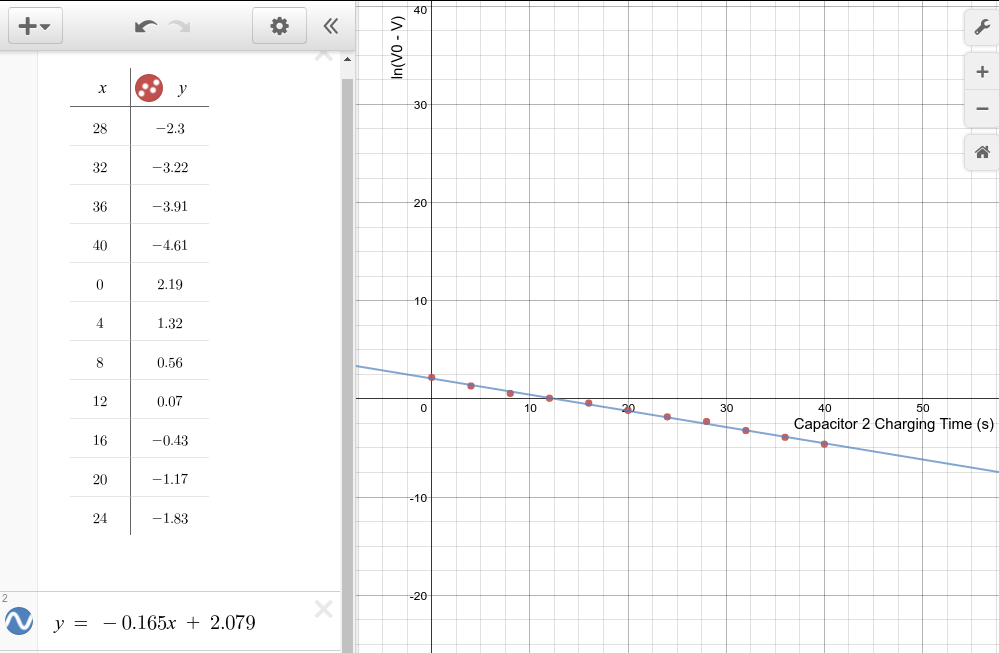
\includegraphics[scale=0.45]{graph33.jpg}
\vspace*{0cm}
\end{figure}

\begin{figure}[h]
\centering
\hspace*{0cm}
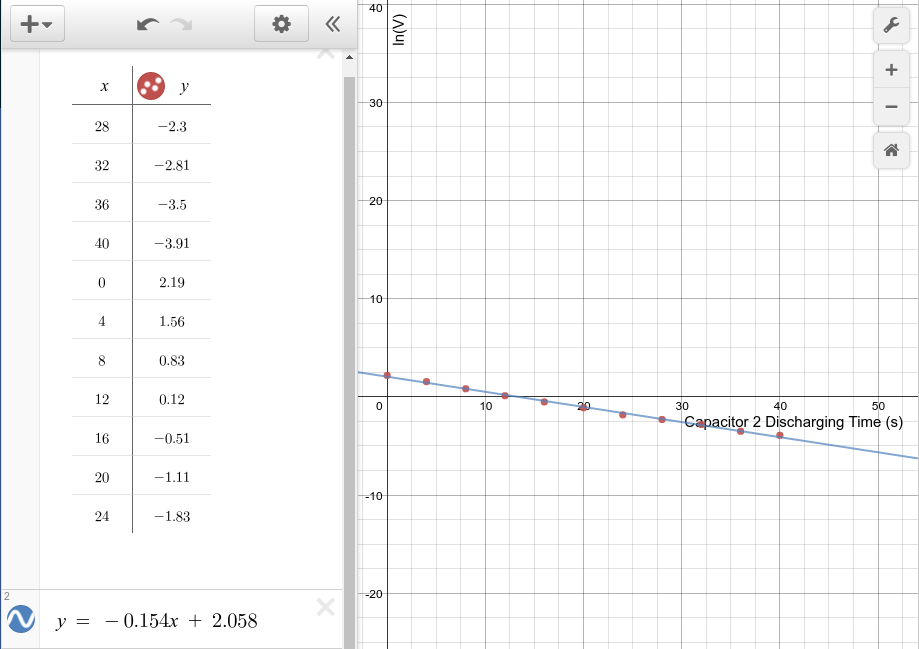
\includegraphics[scale=0.5]{graph34.jpg}
\vspace*{0cm}
\end{figure}

The most likely cause of error is the inaccuracy of measuring such rapid change in the voltmeter reading, both due to the limitation of the voltmeter measurement rate itself, as well as in the human capacity of record the change quickly enough. In addition, since the wires themselves are not ideal, there is some resistance from that, such that the measured RC value would be likely higher than the calculated value, due to the added in series resistance of the wire. In addition, the non-ideal voltmeter most likely would not have an infinitely high resistance, changing the flow of current.

\section*{Conclusion}

The capacitor with a capacitance of 4200 $\mu F$ with a resistor of 1350 $\Omega$ measured an RC constant of 6.27 F*s to the actual RC of 5.67 F*s, with a percent error of 10.6\%. The capacitor with a capacitance of 5100 $\mu F$ with a resistor of 1350 $\Omega$ measured an RC constant of 9.174 F*s to the actual RC of 6.885 F*s, with a percent error of 33.2\%.

\end{document}
